\subsection{Motherboard}

Una vegada escollits dos processadors com a contrincants, hem començat a mirar quines plaques bases hi havia al mercat. Primerament, les hem anat buscant de manera individual i les que hem seleccionat es poden veure a la taula següent.

% Please add the following required packages to your document preamble:
% \usepackage[table,xcdraw]{xcolor}
% If you use beamer only pass "xcolor=table" option, i.e. \documentclass[xcolor=table]{beamer}
\begin{table}[H]
\begin{tabular}{|l|l|l|l|l|l|l|}
\hline
\rowcolor[HTML]{C0C0C0} 
Nom & \begin{tabular}[c]{@{}l@{}}Max \\ Cores\end{tabular} & \begin{tabular}[c]{@{}l@{}}Storage\\ Speed\end{tabular} & \begin{tabular}[c]{@{}l@{}}Max\\ DIMS\end{tabular} & \begin{tabular}[c]{@{}l@{}}USB\\  3.0\end{tabular} & PCI-E & Preu \\ \hline
H12DSU-iN \cite{mother1} & 64 & 6 Gbps & 32 & 5 & 1x16, 1x32, 1x40 & Coming soon \\ \hline
H12DST-B \cite{mother2} & 64 & 6 Gbps & 16 & 2 & 3x16, 1x24 & - \\ \hline
H12SSW-NT \cite{mother3} & 64 & 6 Gbps & 8 & 7 & 1x16, 1x32 & 1356.53\euro \cite{mother3_preu}\\ \hline
H12SSW-iN \cite{mother4} & 64 & 6 Gbps & 8 & 7 & 2x32 & - \\ \hline
H12SST-PS \cite{mother5} & 64 & 6 Gbps & 8 & 2 & 3x16 & 3959.86\euro \cite{mother5_preu}\\ \hline
\end{tabular}
\caption{Comparació inicial de motherboards}
\end{table}

Com es pot veure, les diferències principals son el número de DIMS de memòria i els PCI-Express. No obstant, una vegada fetes les comparacions inicials, ens hem adonat que per algunes d'elles era excessivament complicat trobar el preu. Per exemple, els llocs on trobàvem els preus no és el mateix que on trobàvem les especificacions, per tant en alguns no estem segurs de que els preus siguin del tot realistes.

Buscant els preus ens hem trobat amb una altra web \cite{webnodes} que ens permet crear un node seleccionant nosaltres els seus components. Hem vist que els tipus de node es diferencien inicialment entre aquells amb GPU i aquells sense GPU. Dins d'aquests dos grups, trobem també els dual-socket i els single-socket.

\begin{figure}[H]
    \centering
    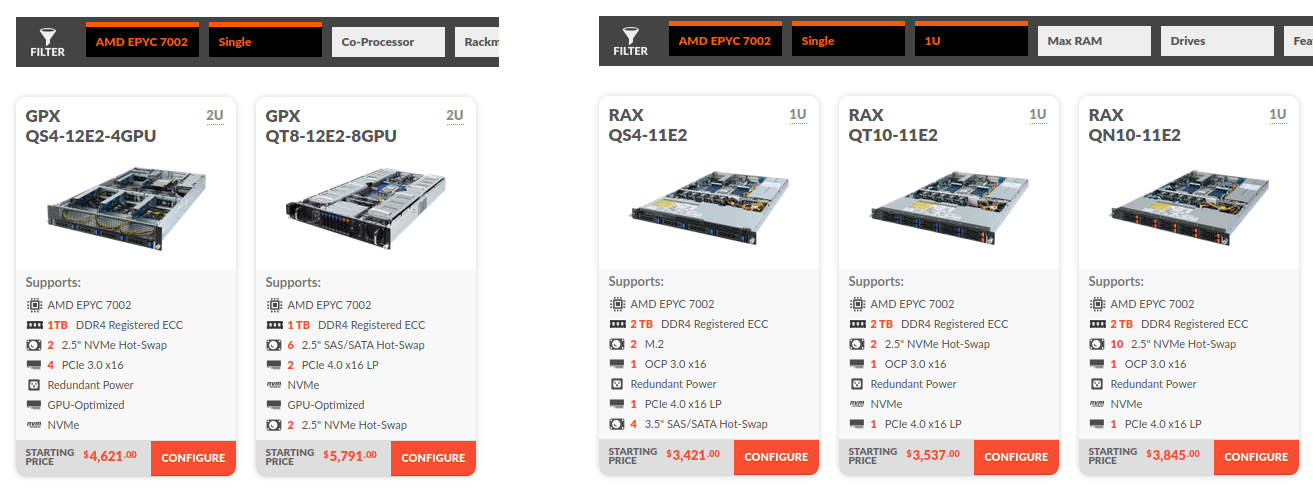
\includegraphics[width=\textwidth]{img/webnodes.png}
    \caption{Exemple de nodes que podem trobar a la web. A l'esquerra amb GPUs i a la dreta sense. Tots single-socket.}
\end{figure}

Com que el processador \textit{AMD EPYC 7702P} té seixanta-quatre nuclis i l'\textit{AMD EPYC Rome 7502P} en té trenta-dos, hem decidit plantejar-nos les opcions de nodes dual-socket amb dos processadors \textit{7502P} i nodes single-socket amb el processador \textit{7702P}. En cas d'escollir un node amb suport per GPU, ocuparem dues \textit{U}s en compte d'una de sola. En el cas dels nodes amb dual-socket, es poden suportar fins a vuit GPUs mentre que amb els single-socket només la meitat, quatre.

 En la següent taula es veuen aquestes possibles combinacions. En el cas d'utilitzar un node amb GPUs no s'ha inclòs el preu de la pròpia GPU, ja que això dependrà de quina escollim més endavant. Per la mateixa raó, tampoc s'han exposat els GFLOPs de les versions amb GPU. En aquests preus tampoc s'inclouen els costos de les memòries i les targetes de xarxa.

\begin{table}[H]
\begin{tabular}{|c|c|c|c|c|c|c|}
\hline
\rowcolor[HTML]{C0C0C0} 
\multicolumn{1}{|l|}{\cellcolor[HTML]{C0C0C0}Configuració} & \multicolumn{1}{l|}{\cellcolor[HTML]{C0C0C0}\#cores} & \multicolumn{1}{l|}{\cellcolor[HTML]{C0C0C0}\begin{tabular}[c]{@{}l@{}}GFLOPs\\  CPU\end{tabular}} & \multicolumn{1}{l|}{\cellcolor[HTML]{C0C0C0}\#GPUs} & \multicolumn{1}{l|}{\cellcolor[HTML]{C0C0C0}Us} & \multicolumn{1}{l|}{\cellcolor[HTML]{C0C0C0}Preu} & \multicolumn{1}{l|}{\cellcolor[HTML]{C0C0C0}GFLOPS/\euro} \\ \hline
\cellcolor[HTML]{EFEFEF} &  &  & - & 1 & 10001 & 0.256 \\ \cline{4-7} 
\multirow{-2}{*}{\cellcolor[HTML]{EFEFEF}\begin{tabular}[c]{@{}c@{}}Dual amb AMD\\ EPYC Rome 7502P\end{tabular}} & \multirow{-2}{*}{128} & \multirow{-2}{*}{2560} & 8 & 2 & 12266 & - \\ \hline
\cellcolor[HTML]{EFEFEF} &  &  & - & 1 & 8172 & 0.251 \\ \cline{4-7} 
\multirow{-2}{*}{\cellcolor[HTML]{EFEFEF}\begin{tabular}[c]{@{}c@{}}Single amb AMB\\ EPYC 7702P\end{tabular}} & \multirow{-2}{*}{128} & \multirow{-2}{*}{2048} & 4 & 2 & 9461 & - \\ \hline
\end{tabular}
\caption{Comparació entre les diferents configuracions dels nodes}
\end{table}

Veiem que tot i que la versió amb dual socket ens proporciona més GFLOPs, l'eficiència GFlops/euro és millor per la versió amb single socket. Per tant, en aquest punt encara no podem decantar-nos per cap de les dues. Una vegada haguem considerat quines GPUS utilitzem, quina xarxa tenim, etc. podrem valorar si tenim suficient presupost com per escollir la opció amb més GFLOPS. Alhora, quan les GPUs entrin en joc també s'haurà de tenir en compte que amb la opció dual-socket en podem possar el doble per cada node.

